\documentclass[11pt]{article}

\usepackage[margin=1in]{geometry}
\usepackage[T1]{fontenc}
\usepackage[utf8]{inputenc}
\usepackage{lmodern}
\usepackage{amsmath,amssymb,amsthm}
\usepackage{booktabs}
\usepackage{tabularx}
\usepackage{array}
\usepackage{longtable}
\usepackage{enumitem}
\usepackage{xcolor}
\usepackage{graphicx}
\graphicspath{{figures/}{docs/overview/figures/}}
\usepackage[colorlinks=true,linkcolor=blue!60!black,citecolor=blue!60!black,urlcolor=blue!60!black]{hyperref}

\setlist{itemsep=2pt,topsep=4pt}
\setlength{\parskip}{4pt}
\renewcommand{\arraystretch}{1.15}
\newcolumntype{L}{>{\raggedright\arraybackslash}X}
\newcolumntype{R}{>{\raggedleft\arraybackslash}X}

\newtheorem{proposition}{Proposition}
\newtheorem{lemma}[proposition]{Lemma}
\newtheorem{conjecture}{Conjecture}
\newtheorem*{fact}{Fact}
\theoremstyle{definition}
\newtheorem*{definition}{Definition}
\theoremstyle{remark}
\newtheorem*{remark}{Remark}

\newcommand{\Eo}{\textsf{E0}}
\newcommand{\Em}{\textsf{E1m}}
\newcommand{\ms}{\,\text{ms}}
\newcommand{\sx}{\,\text{s}}
\newcommand{\file}[1]{\texttt{#1}}
\newcommand{\E}{\mathbb{E}}
\newcommand{\one}{\mathbf{1}}
\newcommand{\todo}[1]{\textcolor{red!70!black}{[#1]}}
\newcommand{\done}{\textcolor{green!45!black}{$\checkmark$}}
\newcommand{\open}{$\square$}

\title{When to execute: order timing under multi-timescale Hawkes intensities of mid-price moves\\[6pt]
\large Project overview: background, model, research questions, results so far, and work to be done}
\author{Hyoeun Lee}
\date{October 9, 2026}

\begin{document}
\maketitle

\begin{abstract}
\noindent
A trader who must buy within a deadline can buy now or wait. If the price process has short-term predictable structure, waiting has value when the price is expected to fall and a cost when it is expected to rise. This project asks what that value is when the predictable structure is the clustering of mid-price moves in liquid US stocks, modelled by a Hawkes process with several timescales. The starting point is the bivariate (up/down) Hawkes model with a sum of $K$ exponential kernels fitted in our companion project to clean mid-price moves from consolidated TAQ data. Writing the excitation of each component as self-excitation $a_k$ and cross-excitation $c_k$, the difference $g_k = a_k - c_k$ (the \emph{signed kernel}) is all that drives the expected direction of future moves; the state of the problem is the vector of $K$ \emph{signed accumulators}, one per timescale, and the expected price displacement over any horizon is a linear function of that state with a closed form. We show that the expected long-run displacement after an up move is $G/(1-G)$ ticks per tick, where $G = \sum_k g_k$; that the rule ``buy as soon as the price is not expected to fall before the deadline'' is a half-space in the state whose normal vector turns as the deadline approaches; and that this rule is monotone in each signed accumulator when $\sum_k |g_k| < 1/2$. On INTC in May 2017, with a kernel fitted on April, this rule saves 0.040 ticks per order at random decision times (deadline 60 seconds, 8\% of the half-spread) and 0.155 ticks after up moves (31\%), and the result does not depend on execution latency between 0 and 2 milliseconds. A rule driven by raw quote changes does better at zero latency, but its advantage comes from brief locked states that resolve within a millisecond and is gone at 2 milliseconds of latency; at that latency it pays 0.42 ticks after raw up moves. A rule that uses only the current intensity difference, as a one-timescale model would, saves a third less at random times, nothing after up moves, and pays ten times as much after down moves. This document sets out the background (market structure, Hawkes processes, optimal execution and optimal stopping of piecewise-deterministic processes), the data, the model and its derivations, the research questions, every result obtained so far, the weaknesses, and the work still to be done.
\end{abstract}

\tableofcontents
\newpage

%==========================================================================
\section{The project in one page}
\label{sec:onepage}

\paragraph{The question.} A trader must buy one unit of a stock within $T$ seconds (sell is the mirror image). She can send a marketable order now, or wait. When should she buy? If prices were a martingale it would not matter. Prices of liquid stocks are not a martingale at the shortest horizons: mid-price moves cluster and partly reverse, and a Hawkes process with several timescales describes this well (our companion project, \emph{hawkes-taq}). The question is how much this predictability is worth to a trader who acts on it in real time, which parts of it survive realistic latency, and what the optimal rule looks like.

\paragraph{The model.} Up and down moves of the mid-price follow the bivariate Hawkes process of hawkes-taq: a shared baseline $\mu(t)$, and a kernel that is a sum of $K = 4$ exponentials with memories of about $10\ms$, $0.1\sx$, $2\sx$ and $40\sx$. Component $k$ has self-excitation $a_k$ (an up move triggers up moves) and cross-excitation $c_k$ (an up move triggers down moves).

\paragraph{The key reduction (Section~\ref{sec:model}).} Only the difference $g_k = a_k - c_k$ matters for the expected direction. The baseline cancels, and the expected signed displacement of the mid over any horizon is a linear function of $K$ \emph{signed accumulators} $d_k(t)$, each an exponentially weighted sum of past moves (up $+1$, down $-1$) at timescale $k$:
\[
\E\big[\text{mid}(t+H) - \text{mid}(t) \,\big|\, \mathcal F_t\big] = \text{size}\cdot g^\top\!\!\int_0^H\! e^{Ms}\,ds\; d(t), \qquad M = -\operatorname{diag}(\beta) + \beta g^\top .
\]
After an isolated up move the expected total displacement is $G/(1-G)$ moves, $G = \sum_k g_k$ (Proposition~\ref{prop:longrun}). In the fitted models $g_k$ changes sign across timescales: INTC continues at $15\ms$ and reverses at seconds to a minute; TGT continues at $5\ms$, reverses at $40\ms$, and continues again at $10\sx$.

\paragraph{The stopping problem (Section~\ref{sec:stopping}).} Minimizing the expected price paid is optimal stopping of a piecewise-deterministic Markov process (PDMP) with a running cost linear in $d$. So far we use a one-step rule: buy as soon as the price is not expected to fall any further before the deadline. Its stopping region is a half-space in $d$ whose normal vector turns as the deadline approaches, so it is not a threshold in the current intensity difference unless $K = 1$. It is monotone in each $d_k$ when $\sum_k|g_k| < 1/2$ (Proposition~\ref{prop:sign}), which holds in every fit so far.

\paragraph{Results so far (Section~\ref{sec:results}).} INTC and TGT, April--May 2017; costs are the quoted ask paid minus the ask at the decision, in ticks.
\begin{enumerate}
\item \textbf{Out of sample, timing has value.} INTC, kernel fitted on April, tested on May, $1\ms$ confirmation delay, $2\ms$ execution latency: at random decision times the rule saves $0.040$ ticks (SE $0.011$) with a $60\sx$ deadline; after up moves it saves $0.155$ ($0.028$); after down moves it buys at once and avoids the $+0.21$ ticks that waiting costs.
\item \textbf{The value is latency-free.} Execution latency of $0$ against $2\ms$ changes the clean rule's costs by under $0.002$ ticks; the $1\ms$ event-confirmation delay changes them by up to $0.02$.
\item \textbf{Raw quote changes give a latency race, not a forecast.} The rule driven by raw NBBO changes saves $0.19$ ticks at random times with zero latency, $0.15$ at $0.5\ms$ and $0.03$ at $2\ms$; after raw up moves it pays $+0.42$ ticks at $2\ms$. Its edge is the second half of a move through a lock, visible for well under a millisecond.
\item \textbf{The timescale decomposition matters for the decision.} The rule that uses only the sign of the current intensity difference saves $0.026$ ticks at random times (against $0.040$), nothing after up moves (against $0.155$), and pays $0.073$ after down moves (against $0.007$).
\item \textbf{The fastest signed component is not stable across months.} INTC's $g_1$ is $+0.060$ in April and $+0.019$ in May; the April model predicts a continuation of $0.05$ ticks at $0.1\sx$ that May does not show (Figure~\ref{fig:response}). The slower components carry the value.
\end{enumerate}

\paragraph{Next.} The out-of-sample panel for all eight stocks and both directions (job ready), the optimal rule against the one-step rule, the signed kernel across all 112 fitted stock-months, and proofs for the optimal rule (Section~\ref{sec:todo}).

%==========================================================================
\section{Background}
\label{sec:background}

This section collects the background needed for the rest. The market and Hawkes material is covered in more detail in the hawkes-taq overview; it is repeated here only as far as needed.

\subsection{Large-tick stocks, the spread, and the NBBO}
\label{sec:bg-market}

US stocks trade in a limit order book on each of about a dozen exchanges. The \emph{best bid} is the highest price at which someone has offered to buy, the \emph{best ask} the lowest price at which someone has offered to sell, and the \emph{spread} their difference. Prices move on a grid of one cent, the \emph{tick}. A stock is \emph{large-tick} when the tick is large relative to its price and volatility, so that the spread sits at its one-tick minimum almost all the time; the core stocks here (INTC, MU, MDLZ, BAC, WFC, T) spend at least 99.8\% of the time at one tick. The \emph{mid-price} is the average of the best bid and ask. At a one-tick spread, a change in the mid is a change of both quotes, and the ask paid by a buyer moves one for one with the mid.

The \emph{national best bid and offer} (NBBO) combines the best quotes of all exchanges. It is computed by the consolidated feed (the SIP) and recorded with microsecond timestamps in WRDS Millisecond TAQ. Because exchanges update at slightly different times and the feed has its own latency, about half of NBBO changes in large-tick stocks are \emph{brief states} that last well under a millisecond, mostly \emph{locks} where the best bid equals the best ask. A typical price move goes one tick $\to$ locked $\to$ one tick at the new level. The hawkes-taq project measures this in detail; for us it matters in two ways. First, the event series must be built so that each persistent price move counts once (definition \Em, Section~\ref{sec:events}). Second, the brief states carry information: a lock where the bid has risen to the ask is usually followed within a millisecond by the ask rising. That information is real but available only to a trader fast enough to act within the lock (Section~\ref{sec:res-raw}).

\subsection{Point processes and Hawkes processes}
\label{sec:bg-hawkes}

A \emph{point process} is a random set of event times; a \emph{multivariate} point process also records a type. Its \emph{conditional intensity} $\lambda_i(t)$ is the instantaneous rate of type-$i$ events given the history. A \emph{Hawkes process} (Hawkes, 1971) has intensity
\[
\lambda_i(t) = \mu_i(t) + \sum_j \sum_{t^j_m < t} \phi_{ij}(t - t^j_m),
\]
so each event raises future intensities. With exponential components $\phi_{ij}(s) = \sum_k \alpha_{ij,k}\beta_k e^{-\beta_k s}$, each component integrates to $\alpha_{ij,k}$ (the expected number of type-$i$ events directly triggered by one type-$j$ event through component $k$), its \emph{memory} is $1/\beta_k$, and the sum over the past obeys an $O(N)$ recursion (Ozaki, 1979). The \emph{branching ratio}, the spectral radius of the matrix of total excitation, must be below 1 for stationarity (Hawkes, 1971; Br\'emaud and Massouli\'e, 1996). Sums of exponentials approximate the slowly decaying kernels found in financial data (Hardiman, Bercot and Bouchaud, 2013; Bacry, Jaisson and Muzy, 2016; Lallouache and Challet, 2016; Kyungsub Lee, 2023). For mid-price moves, two mutually exciting types (up and down) were introduced by Bacry, Delattre, Hoffmann and Muzy (2013), and the symmetric form we use, with equal self-excitation for both directions and equal cross-excitation, is that of Lee and Seo (2017). Cross-excitation from up to down moves is how these models produce the mean reversion of prices at short horizons (``microstructure noise''); self-excitation produces trends. Their balance, component by component, is the object of this project.

\subsection{Optimal execution}
\label{sec:bg-exec}

Optimal execution asks how to buy or sell a given quantity over a horizon at the least expected cost, usually traded off against risk. The classical model (Almgren and Chriss, 2001) splits a large order over time against permanent and temporary price impact. Models of the limit order book add the choice between limit orders (better price, uncertain fill) and market orders (certain fill, pay the spread) and the management of inventory (Avellaneda and Stoikov, 2008; Gu\'eant, Lehalle and Fernandez-Tapia, 2013; textbook treatments in Cartea, Jaimungal and Penalva, 2015, and Gu\'eant, 2016). Order-flow and price signals enter as drifts: a trader who knows that the price is likely to rise should buy sooner (Cartea, Jaimungal and Ricci, 2014; Bank, Cartea and K\"orber, 2023).

Hawkes processes appear in this literature as models of order flow. Alfonsi and Blanc (2016) solve optimal execution when other traders' market orders follow a Hawkes process and move the price through transient impact. Cartea, Jaimungal and Ricci (2014) let market-order arrivals be self-exciting in a market-making problem. Chevalier, Hafsi and Ly Vath (2024) use mutually exciting Hawkes order flow with a hidden liquidity state and solve the liquidation problem as impulse control. Chatziandreou and Karbach (2025) apply a bivariate Hawkes order-flow model with transient impact to intraday electricity markets. Lehalle and Mounjid (2016) study how latency limits the value of predicting order flow when placing limit orders.

What these papers do not do, as far as we have found, is take a fitted multi-timescale Hawkes model of \emph{price moves} as the predictive state and ask how the timescale structure of its signed excitation shapes the decision. The closest is the signal-driven execution of Bank, Cartea and K\"orber (2023), where a short-term signal of order flow enters the trader's control problem; there the signal is exogenous, while here it is the model's own filtered state, with a structure (several timescales of opposite sign) that a single signal does not have.

\subsection{Optimal stopping and piecewise-deterministic Markov processes}
\label{sec:bg-stopping}

An \emph{optimal stopping problem} chooses a stopping time $\tau$ (a random time decided on information available up to it) to minimize $\E[C_\tau]$ for a cost process $C$. For a Markov state $X$ and $C_\tau = \int_0^\tau f(X_s)\,ds$, the value function $V(x) = \inf_\tau \E_x[C_\tau]$ is the smallest solution of a dynamic programming principle; the optimal rule stops on the \emph{stopping region} $\{V = 0\}$ (stopping now costs nothing more) and continues on $\{V < 0\}$. Peskir and Shiryaev (2006) is the standard reference for the continuous-time theory.

A \emph{piecewise-deterministic Markov process} (PDMP; Davis, 1984, 1993) moves along a deterministic flow between random jump times; the jump rate and the jump distribution depend on the state. The state of an exponential-kernel Hawkes process (its accumulators) is a PDMP: it decays exponentially between events and jumps at events. Optimal stopping of PDMPs reduces to iterating a \emph{single-jump operator} (Gugerli, 1986): between jumps the path is deterministic, so each step is a one-dimensional minimization over the stopping time before the next jump. Costa and Davis (1988) gave approximation schemes, and de Saporta, Dufour and Gonzalez (2010) a numerical method based on quantization with error bounds. Section~\ref{sec:stopping-pdmp} writes our problem in this form.

\subsection{Latency}
\label{sec:bg-latency}

A trader observes the market with a delay and acts with a delay. In consolidated data the delay between an exchange's clock and the SIP's is about $0.02\ms$ for Nasdaq venues, $0.2\ms$ for Cboe and $0.4\ms$ for NYSE Arca (hawkes-taq data checks); the trader's own round trip adds to this. Lehalle and Mounjid (2016) show that forecasting order flow is worth less to a slower trader. Our setting gives a sharp version: the predictive content of the consolidated quotes splits into a part that lives in sub-millisecond brief states and a part that lives in the clustering of persistent moves, and only the second is available to a trader with a few milliseconds of latency (Section~\ref{sec:res-raw}).

%==========================================================================
\section{Where this project comes from}
\label{sec:origins}

\subsection{The spread-gated Hawkes-flocking paper}

Lee and Lee (2026) model the four best-quote moves (ask up, ask down, bid up, bid down) with the spread as a state variable: spread-narrowing moves are switched off at one tick, and a cross-side ``flocking'' kernel is switched on according to the current spread. Fitted to one day of LOBSTER data for INTC and MSFT, the flocking kernel's role is a millisecond snap-back of the spread after a widening. The paper closes with a single-period limit-order placement rule whose execution probabilities are assumed (0.7 and 0.5), and names three directions for further work: estimating the execution probabilities, a multi-period strategy, and better-fitting kernels (the fitted model is rejected by Kolmogorov--Smirnov tests and generates 1,337 widening events against 884 observed for INTC).

This project is the multi-period direction. It started from the flocking model's four-type state and moved to the mid-price model for three reasons. (i) On consolidated data the two-tick windows in which the flocking kernel acts are among the brief states that \Em{} merges; a stopping rule that acts inside them is the latency race of Section~\ref{sec:res-raw}. (ii) The mid-price model has been fitted, with multi-timescale kernels and bootstrap standard errors, to eight stocks over 14 months, and its signed price path after an event matches the data (hawkes-taq results, section 19). (iii) The drift of the mid-price model reduces to the $K$ signed accumulators (Section~\ref{sec:model}), which makes the stopping problem tractable. The resting-order problem, in which the spread state and the flocking mechanism matter, is kept as an extension (Section~\ref{sec:resting}); it is where the flocking paper's assumed execution probabilities become model outputs.

\subsection{The hawkes-taq project}

Hawkes-taq fits the symmetric bivariate model of Section~\ref{sec:model} to mid-price moves built from WRDS TAQ NBBO changes for eight stocks, November 2016 -- December 2017 (291 trading days), comparing event definitions. Results used here:

\begin{itemize}
\item On clean events (\Em: states shorter than $1\ms$ merged, $1\ms$ refractory period in the fit), BIC prefers $K = 4$ in 103 of 112 stock-months (BAC: $K = 3$). Core-stock memories are about $10$--$13\ms$, $60$--$140\ms$, $1.5$--$2.6\sx$ and $30$--$40\sx$; TGT and ATVI have the same shape compressed by a factor of 2--3.
\item The clean model reproduces the signed mid-price path after an event within $0.025$ ticks up to one second; the raw-event (\Eo) model implies about twice the continuation that occurs (hawkes-taq results, section 19).
\item Kernel mass within $1\sx$ and $10\sx$ is precisely estimated and stable across baseline specifications; the total branching ratio and the slowest component are not (bias of about $-20\%$ in the bootstrap; sensitivity to the baseline bin width; sections 15--16).
\item An \Em{} event is confirmed only once its new state has lasted $1\ms$; any real-time use must respect this (external review, point F).
\end{itemize}

The fitted parameters $a_k$ (self) and $c_k$ (cross) for all 112 stock-months are already saved in the hawkes-taq panel results, so the signed kernel can be studied across the whole panel without refitting (Section~\ref{sec:todo}).

\subsection{Formulations considered}
\label{sec:formulations}

Before settling on the problem of Section~\ref{sec:stopping}, several readings of ``stopping with Hawkes intensities'' were considered.

\begin{center}
\begin{tabularx}{\textwidth}{@{}p{3.6cm}LL@{}}
\toprule
Formulation & What it is & Status \\
\midrule
Marketable-order timing & Buy within a deadline; stop when the expected remaining price change is unfavourable & \textbf{Main problem (P1)} \\
Resting-order timing & Keep, cancel or cross a resting limit order; fill probabilities from the model & Extension (P2), needs queue sizes \\
Regime detection & Detect a shift in intensity (quickest detection, CUSUM/Shiryaev type) with the Hawkes accumulator as statistic & In reserve: a natural fallback if P1's value were negligible \\
Sequential learning & Stopping with unknown kernel parameters, learned online & Later: Section~\ref{sec:res-stability} shows month-to-month instability of $g_1$, which motivates it \\
Online / secretary-type & Worst-case (prophet) guarantees without a model & Set aside: discards the predictive model, which is the point \\
\bottomrule
\end{tabularx}
\end{center}

%==========================================================================
\section{Research questions}
\label{sec:rq}

\begin{description}[leftmargin=0pt]
\item[RQ1 (Structure).] What does the optimal rule for P1 look like in the signed-accumulator state? Is the stopping region monotone in each $d_k$? How far is it from the one-step rule, whose region is a half-space with a turning normal (Proposition~\ref{prop:sign})? How does the unsigned state (activity), which does not enter the drift, enter the optimal rule through the option value of waiting?
\item[RQ2 (Value).] What is timing worth, in ticks and as a share of the half-spread, by stock, deadline, decision context (random time, after an up move, after a down move) and side, out of sample?
\item[RQ3 (Latency).] How does the value decay with execution latency, for rules driven by raw and by clean events? The difference measures how much short-horizon predictability in consolidated quotes is a latency race in brief states, and how much is latency-free.
\item[RQ4 (Which parts of the kernel matter).] The decision with deadline $T$ depends on the kernel mainly through its signed mass within $T$. Are the components that carry the value the ones that are well identified and stable across months (hawkes-taq sections 15--16)? How much does a one-timescale model lose?
\item[RQ5 (Robustness).] The clean model is rejected by calibrated goodness-of-fit tests. How much of the rule's value survives misspecification: alternative kernels (full asymmetric, power-law), baseline specifications, $K = 3$ against $K = 4$, and the refractory period? Is the value larger on data simulated from the fitted model than on the real data (an estimate of what misspecification costs)?
\end{description}

\noindent\textbf{Headline:} RQ1 (a structural result) and RQ3 (an empirical decomposition with a clear message). RQ2 provides the magnitudes; RQ4 and RQ5 make the conclusions robust.

%==========================================================================
\section{Data}
\label{sec:data}

\subsection{Source and sample}

\begin{center}
\begin{tabularx}{\textwidth}{@{}p{3.3cm}L@{}}
\toprule
Item & Choice \\
\midrule
Source & WRDS Millisecond TAQ, \file{taqmsec.complete\_nbbo\_YYYYMMDD} (the completed NBBO table, which includes quotes missing from \file{nbbom}); microsecond timestamps (\file{time\_m}, SIP time) \\
Stocks & Core large-tick: INTC, MU, MDLZ (Nasdaq-listed); BAC, WFC, T (NYSE-listed). Contrast: TGT, ATVI (more active; less time at one tick in parts of the sample) \\
Collected & All eight stocks, Oct 31, 2016 -- Dec 29, 2017 (hawkes-taq); 2017Q2 (Apr 3 -- Jun 30, 63 trading days, all eight stocks) in hand for this project \\
Used so far & INTC: April (19 days) and May (22 days) 2017; TGT: May 2017 \\
Window & 10:00--15:30 each day; early-close days excluded \\
Clock & SIP time; exchange time is available for a sensitivity check (hawkes-taq builds an exchange-timestamp reconstruction) \\
\bottomrule
\end{tabularx}
\end{center}

The only WRDS step saves the NBBO price changes of one stock-day: the rows where the best bid or best ask differs from the previous row, with columns \file{t} (seconds after midnight), \file{bid}, \file{ask}. The query (hawkes-taq, \file{hawkes\_taq/fetch.py}) is
\begin{verbatim}
with q as (
    select time_m, best_bid, best_ask,
           lag(best_bid) over w as pb, lag(best_ask) over w as pa
    from taqmsec.complete_nbbo_{date}
    where sym_root = '{sym}' and sym_suffix is null
      and time_m between '10:00:00' and '15:30:00'
      and best_bid > 0 and best_ask > 0
    window w as (order by time_m)
)
select time_m, best_bid, best_ask from q
where pb is null or best_bid <> pb or best_ask <> pa
order by time_m
\end{verbatim}
Everything else (states, events, fits, backtests) runs outside WRDS. TAQ-derived files (NBBO changes, events, fitted models, per-day results) stay out of the repository; only aggregate results are committed.

\begin{center}
\begin{tabularx}{\textwidth}{@{}lrRRRRr@{}}
\toprule
Stock & Clean events/day & Memory 1 & Memory 2 & Memory 3 & Memory 4 & Eff.\ BR \\
\midrule
INTC & 830 & 12.7\ms & 136\ms & 2.6\sx & 39\sx & 0.46 \\
MU & 1,755 & 12.0\ms & 74\ms & 1.9\sx & 37\sx & 0.53 \\
MDLZ & 1,161 & 5.2\ms & 62\ms & 1.6\sx & 29\sx & 0.56 \\
BAC ($K=3$) & 700 & 9.3\ms & 102\ms & 27\sx & --- & 0.33 \\
WFC & 2,065 & 11.5\ms & 76\ms & 1.5\sx & 28\sx & 0.51 \\
T & 688 & 11.1\ms & 117\ms & 2.2\sx & 40\sx & 0.40 \\
TGT & 3,997 & 3.8\ms & 39\ms & 0.86\sx & 11\sx & 0.65 \\
ATVI & 3,943 & 2.7\ms & 30\ms & 0.81\sx & 12\sx & 0.64 \\
\bottomrule
\end{tabularx}
\end{center}
\noindent{\small Sample stocks: median over 14 months of clean (\Em) events per day and of the main hawkes-taq fits ($K = 4$, $1\ms$ refractory period; effective branching ratio). From hawkes-taq results, sections 3 and 12. A fastest memory under about $6\ms$ is not resolved by the $1\ms$ cleaning threshold (hawkes-taq section 14).}

\subsection{States and events}
\label{sec:events}

Prices are converted to integer ticks. Consecutive NBBO changes define \emph{states} with a bid, an ask, a spread and a duration. Two event definitions are used (hawkes-taq, \file{hawkes\_taq/events.py}):

\begin{description}[leftmargin=0pt]
\item[\Eo{} (raw).] Every NBBO change that moves the mid. About half are brief states and their resolutions; typical size half a tick (mean $0.50$).
\item[\Em{} (clean, main).] Mid-price moves after merging every state shorter than $h = 1\ms$, and locked or crossed states shorter than $5\ms$, into the move around them. A move that passes through such a state counts once, stamped when the new level is first quoted (exit of the brief state). Almost all \Em{} moves are one tick (mean size $0.93$--$0.96$ ticks). The new level is known to persist only once it has lasted $h$, so in real time an \Em{} event at $t$ is \emph{confirmed} at $t + h$.
\end{description}

\noindent Event counts in the months used: INTC April 16,475 \Em{} events (19 days); INTC May 15,888 \Em{} and 32,710 \Eo{} (22 days); TGT May 58,818 \Em{} (22 days). These reproduce hawkes-taq exactly.

\subsection{Execution price}

A buyer pays the ask. Costs are measured on the quoted NBBO ask at execution, in ticks, relative to the ask at the decision time, from the full state sequence (not from events), so they include brief states. Caveats: the order is for one unit (no depth or impact); during a lock the consolidated ask may not be accessible at the quoted price; SIP latency (Section~\ref{sec:bg-latency}) means the quoted ask can be slightly stale.

%==========================================================================
\section{Model}
\label{sec:model}

\subsection{The Hawkes model of mid-price moves}

Events are mid-price moves of sign $\varepsilon_m \in \{+1, -1\}$ (up, down) at times $t_m$. With $N_+$ and $N_-$ the counting processes of up and down moves, the intensities are
\begin{equation}
\lambda_\pm(t) = \mu(t) + \sum_{k=1}^K \beta_k \sum_{t_m < t} \Big( a_k \one\{\varepsilon_m = \pm 1\} + c_k \one\{\varepsilon_m = \mp 1\} \Big) e^{-\beta_k (t - t_m)} ,
\label{eq:model}
\end{equation}
with decay rates $\beta_1 > \dots > \beta_K$ shared by all pairs, self-excitation $a_k \ge 0$ and cross-excitation $c_k \ge 0$ per component (the symmetric specification: an up move triggers up moves as a down move triggers down moves). The baseline $\mu(t)$ is piecewise constant, one level per day and 30-minute bin, shared by both directions. The fits include a refractory period $\delta = 1\ms$ after each event (both intensities zero), matching the $1\ms$ merge threshold of \Em. One kernel is fitted per stock and calendar month by maximum likelihood, pooling days with no excitation carried between days; the decay rates are profiled out by a multi-start Nelder--Mead search (all grid combinations plus the empirical ladders), and for fixed decay rates the likelihood is concave in $(\mu, a, c)$ (hawkes-taq, \file{hawkes\_taq/hawkes.py}). The branching ratio of~\eqref{eq:model} is $\sum_k (a_k + c_k)$.

\subsection{Signed and unsigned accumulators}

Define for each component the unsigned and signed accumulators
\[
u_k(t) = \beta_k \sum_{t_m < t} e^{-\beta_k (t - t_m)}, \qquad d_k(t) = \beta_k \sum_{t_m < t} \varepsilon_m\, e^{-\beta_k (t - t_m)} .
\]
Writing $\one\{\varepsilon = \pm 1\} = (1 \pm \varepsilon)/2$ in~\eqref{eq:model} gives
\begin{equation}
\lambda_\pm(t) = \mu(t) + \tfrac12 \sum_k (a_k + c_k)\, u_k(t) \pm \tfrac12 \sum_k (a_k - c_k)\, d_k(t) .
\label{eq:decomp}
\end{equation}

\begin{definition}
The \emph{signed kernel} is $g_k = a_k - c_k$, $k = 1, \dots, K$: continuation at timescale $k$ if $g_k > 0$, reversal if $g_k < 0$. Its total $G = \sum_k g_k$ is the \emph{signed branching ratio}, and $\|g\|_1 = \sum_k |g_k|$ its absolute mass. The \emph{signed intensity} is $D(t) = \lambda_+(t) - \lambda_-(t) = g^\top d(t)$; the \emph{total intensity} is $\lambda_+ + \lambda_- = 2\mu(t) + (a + c)^\top u(t)$.
\end{definition}

Three facts follow from~\eqref{eq:decomp}. The baseline does not enter the signed intensity, because it is shared by both directions (separate baselines by direction are not supported by BIC in hawkes-taq, section 6). The signed intensity depends only on the signed accumulators. The total intensity, which sets how often moves occur, depends only on the unsigned accumulators and the baseline. Since $|g_k| \le a_k + c_k$, $\|g\|_1$ is at most the branching ratio, so $\|g\|_1 < 1$ in any stationary fit.

\subsection{The state as a piecewise-deterministic Markov process}

The process $X(t) = (u(t), d(t), t)$ is a PDMP. Between events it follows the flow $\dot u = -Bu$, $\dot d = -Bd$, $\dot t = 1$, with $B = \operatorname{diag}(\beta)$. Up moves occur at rate $\lambda_+(X)$ and move $(u, d) \to (u + \beta, d + \beta)$; down moves occur at rate $\lambda_-(X)$ and move $(u, d) \to (u + \beta, d - \beta)$. The mid-price jumps by the move size with each event. Its generator acting on a smooth function $\varphi(u, d, t)$ is
\[
\mathcal L \varphi = \partial_t \varphi - (Bu)^\top \nabla_u \varphi - (Bd)^\top \nabla_d \varphi + \lambda_+ \big[\varphi(u + \beta, d + \beta, t) - \varphi\big] + \lambda_- \big[\varphi(u + \beta, d - \beta, t) - \varphi\big] .
\]
With the refractory period, both rates are zero for $\delta$ after each event; the state then also carries the time since the last event. The derivations below ignore the refractory period; its effect on realized kernel mass is under 1\% in the core stocks (hawkes-taq results, section 10, and external review point A).

\subsection{Expected signed displacement}

\begin{proposition}[Drift in closed form]
\label{prop:drift}
Let $M = -B + \beta g^\top$ and let each move have size $s$ ticks. For $H \ge 0$,
\[
\E\big[\mathrm{mid}(t + H) - \mathrm{mid}(t) \,\big|\, \mathcal F_t\big] = s\, g^\top W(H)\, d(t), \qquad W(H) = \int_0^H e^{Mr}\,dr .
\]
The expected displacement is linear in the signed accumulators and does not depend on the unsigned accumulators or the baseline.
\end{proposition}

\begin{proof}
Let $y(r) = \E[d(t + r) \mid \mathcal F_t]$. Between events $d$ decays as $-Bd$; at an up (down) move it jumps by $+\beta$ ($-\beta$). Its compensator is therefore $(-Bd + \beta(\lambda_+ - \lambda_-))\,dr = (-Bd + \beta g^\top d)\,dr = Md\,dr$, so $y' = My$ and $y(r) = e^{Mr} d(t)$. The mid changes by $+s$ at up moves and $-s$ at down moves, so its compensator is $s (\lambda_+ - \lambda_-)\,dr = s\, g^\top d\,dr$, and $\E[\mathrm{mid}(t + H) - \mathrm{mid}(t) \mid \mathcal F_t] = s \int_0^H g^\top y(r)\,dr$. Integrability holds because the intensities have finite moments when the branching ratio is below 1.
\end{proof}

The computation uses the eigendecomposition $M = V \Lambda V^{-1}$,
\[
W(H) = V \operatorname{diag}\big((e^{\Lambda_{j}H} - 1)/\Lambda_{j}\big) V^{-1}
\]
(\file{stopping/drift.py}). It is checked against the matrix exponential and against simulated Hawkes cascades in \file{tests/test\_drift.py}. The assumption that the move size does not depend on direction or history is close to true for \Em{} (almost all moves are one tick).

\begin{lemma}[Stability]
\label{lem:stable}
If $\|g\|_1 < 1$ (in particular if the branching ratio is below 1), every eigenvalue of $M$ has negative real part.
\end{lemma}

\begin{proof}
$M$ is a rank-one perturbation of $-B$. For $z \ne -\beta_k$, $\det(zI - M) = \prod_k (z + \beta_k) \cdot \big(1 - \sum_k g_k \beta_k / (z + \beta_k)\big)$. If $\operatorname{Re} z \ge 0$ then $|\beta_k / (z + \beta_k)| \le 1$, so $|\sum_k g_k \beta_k/(z + \beta_k)| \le \|g\|_1 < 1$ and the determinant is not zero. The remaining candidates $z = -\beta_k$ have negative real part.
\end{proof}

\begin{proposition}[Long-run displacement]
\label{prop:longrun}
If $\|g\|_1 < 1$, then as $H \to \infty$
\[
s\, g^\top W(H)\, d \;\longrightarrow\; \frac{s}{1 - G} \sum_k \frac{g_k\, d_k}{\beta_k} .
\]
After an isolated up move ($d = \beta$) the expected total displacement is $s\, G/(1 - G)$.
\end{proposition}

\begin{proof}
By Lemma~\ref{lem:stable}, $W(\infty) = -M^{-1} = (B - \beta g^\top)^{-1}$. By the Sherman--Morrison formula, $(B - \beta g^\top)^{-1} = B^{-1} + B^{-1}\beta g^\top B^{-1} / (1 - g^\top B^{-1}\beta)$. Since $B^{-1}\beta = \one$ and $g^\top \one = G$, $g^\top W(\infty)\, d = g^\top B^{-1} d + G\, g^\top B^{-1} d/(1 - G) = g^\top B^{-1} d / (1 - G)$. With $d = \beta$, $g^\top B^{-1}\beta = G$.
\end{proof}

This is the signed analogue of the familiar fact that one event of a Hawkes process with branching ratio $n$ has $n/(1-n)$ descendants in expectation. The sign of $G$ decides whether, in the long run, a move is followed by continuation ($G > 0$) or reversal ($G < 0$); the individual $g_k$ decide the path to it. Numerically the identity holds to four decimals in every fit (Table~\ref{tab:kernels}).

\subsection{The response function and its sign}

Let $\varphi_g(r) = \sum_j g_j \beta_j e^{-\beta_j r}$ (the signed kernel as a function of the lag). The expected signed rate $\rho(r) = \E[D(t + r) \mid \mathcal F_t]$ that follows from a single unit of $d_k$ at $t$ (all other accumulators zero) solves the renewal equation
\begin{equation}
\rho(r) = g_k e^{-\beta_k r} + \int_0^r \varphi_g(r - v)\, \rho(v)\,dv ,
\label{eq:renewal}
\end{equation}
because each expected net move at time $v$ raises the expected signed intensity at time $r$ by $\varphi_g(r - v)$. Its integral $w_k(H) = s\int_0^H \rho$ is the $k$-th coordinate of $s\, W(H)^\top g$: the effect of $d_k$ on the expected displacement over $H$.

\begin{proposition}[Sign of the response]
\label{prop:sign}
If $\|g\|_1 < 1/2$, then for every $H > 0$ and every $k$ with $g_k \ne 0$, $w_k(H)$ has the sign of $g_k$.
\end{proposition}

\begin{proof}
Iterating~\eqref{eq:renewal}, $\rho = x + \varphi_g * x + \varphi_g * \varphi_g * x + \dots$ with $x(r) = g_k e^{-\beta_k r}$. For causal functions, $\int_0^H |f * h| \le \int_0^H |f| \int_0^H |h|$, and $\int_0^\infty |\varphi_g| \le \|g\|_1$. Hence $\big|\int_0^H \rho - X(H)\big| \le |X(H)| \sum_{n \ge 1} \|g\|_1^n = |X(H)|\, \|g\|_1 / (1 - \|g\|_1)$, where $X(H) = \int_0^H x = g_k (1 - e^{-\beta_k H})/\beta_k$ has the sign of $g_k$. When $\|g\|_1 < 1/2$ the bound is below $|X(H)|$.
\end{proof}

The condition is sufficient, not necessary: in every fit so far the conclusion holds at all $H$ from $0.1\ms$ to $1000\sx$, including the raw-event fit with $\|g\|_1 = 0.55$ (Table~\ref{tab:kernels}). The proposition is about each accumulator separately. The response after an \emph{event}, which raises all accumulators at once ($d = \beta$), is a sum of terms of different signs with different decay rates and can change sign with the horizon: for TGT it is positive up to about $18\ms$, negative until about $32\sx$, and positive after (Section~\ref{sec:res-kernels}).

%==========================================================================
\section{The stopping problems}
\label{sec:stopping}

\subsection{P1: timing a marketable order}
\label{sec:p1}

A trader must buy one unit at a time $\tau \in [t_0, t_0 + T]$, a stopping time for the information she has. She pays the ask $A_\tau$. At a one-tick spread the ask moves with the mid, so, up to the rare times the spread is wider,
\[
A_\tau - A_{t_0} = \mathrm{mid}(\tau) - \mathrm{mid}(t_0), \qquad \E[A_\tau - A_{t_0}] = \E\!\int_{t_0}^{\tau} s\, g^\top d(r)\,dr
\]
by Proposition~\ref{prop:drift} and optional stopping. With a running penalty $\phi \ge 0$ per second of waiting (risk, opportunity cost), the problem in the state $x = (u, d, t)$ with remaining time $\theta$ is
\begin{equation}
V(x, \theta) = \inf_{\tau \le \theta} \E_x\Big[\int_0^\tau \big(s\, g^\top d(r) + \phi\big)\,dr\Big] \;\le\; 0 .
\label{eq:value}
\end{equation}
Stopping at once costs 0. The trader waits while $V < 0$ and buys when $V = 0$. A mean--variance version replaces the running cost by $s\,g^\top d + \eta\, s^2 (\lambda_+ + \lambda_-)$ (the instantaneous variance of the mid is $s^2$ times the total intensity), and then the unsigned accumulators enter the cost too.

\paragraph{Information and latency.} Two delays enter. The \emph{information delay} $\ell_I$: the decision at time $r$ uses events up to $r - \ell_I$; for \Em{} events $\ell_I = h = 1\ms$ (confirmation). The \emph{execution latency} $\ell_E$: an order decided at $r$ executes at the ask quoted at $r + \ell_E$. For $\ell_E > 0$ the cost of stopping at $r$ is $\E[A_{r + \ell_E} - A_{t_0}]$, which adds the expected drift over $[r, r + \ell_E]$ to the problem; with a drift of order $0.01$ ticks per $10\ms$ (Figure~\ref{fig:response}) this is negligible for clean events and decisive for raw events, whose drift is concentrated in the first millisecond.

\subsection{Dynamic programming for a PDMP}
\label{sec:stopping-pdmp}

Between events the state is deterministic: $d(t_0 + r) = e^{-Br} d$, $u(t_0 + r) = e^{-Br} u$. The probability of no event during $[0, r]$ is $e^{-\Lambda(x, r)}$ with
\[
\Lambda(x, r) = \int_0^r \big(2\mu(t_0 + v) + (a + c)^\top e^{-Bv} u\big)\,dv ,
\]
explicit for a piecewise-constant baseline; the running cost along the flow, $\int_0^r s\, g^\top e^{-Bv} d\,dv$, is explicit too. Following Gugerli (1986) and Davis (1993), define for a function $w$ the single-jump operator
\[
(\mathcal J w)(x, \theta) = \inf_{0 \le r \le \theta} \Big\{ \int_0^{r} e^{-\Lambda(x, v)} \Big[ s\, g^\top e^{-Bv} d + \phi + \lambda_+(x_v)\, w(x_v^+, \theta - v) + \lambda_-(x_v)\, w(x_v^-, \theta - v) \Big] dv \Big\},
\]
where $x_v$ is the flow from $x$ after time $v$ and $x_v^\pm$ the state after an up or down move at $x_v$. Here $r$ is the time at which to stop if no event has occurred before it. Starting from $V_0 = 0$ (stop at once), $V_{n+1} = \mathcal J V_n$ is the value of rules that may wait through at most $n$ events; $V_n$ decreases to $V$. \todo{Check the exact form of the operator and the convergence conditions in Gugerli (1986) and Davis (1993, ch.~5) before relying on them.}

\paragraph{Computation.} The state has dimension $2K + 2$ (accumulators, time of day for the baseline bin, remaining time); with $K = 4$ that is ten. Grids are out of the question; candidates are quantization (de Saporta, Dufour and Gonzalez, 2010) and regression Monte Carlo (Longstaff and Schwartz, 2001) on simulated paths from the fitted model. Dimension reduction is available: the fastest component decays within tens of milliseconds and can often be set to zero between events, and the drift depends on $d$ only through $K$ coordinates.

\subsection{The one-step rule used so far}
\label{sec:onestep}

Instead of the optimal rule, the results so far use
\[
\hat\tau = \inf\big\{ r \ge t_0 : m\big(d(r), t_0 + T - r\big) \ge 0 \big\} \wedge (t_0 + T), \qquad m(d, H) = s\, g^\top W(H)\, d ,
\]
that is: buy as soon as the price is not expected to fall any further before the deadline (with $\phi = 0$). It compares stopping now with one alternative, waiting until the deadline, and is therefore suboptimal; its value is a lower bound on the value of timing. It is checked at the start, after every event (once confirmed), and on a grid of 20 points within the deadline (\file{stopping/backtest.py}).

\paragraph{Structure.} The stopping region of the one-step rule at remaining time $H$ is the half-space $\{d : w(H)^\top d \ge 0\}$ with normal $w(H) = s\, W(H)^\top g$.
\begin{itemize}
\item \emph{Monotone in each accumulator.} Under Proposition~\ref{prop:sign} each coordinate $w_k(H)$ has the sign of $g_k$ at every $H$: a larger $d_k$ for a reversal component ($g_k < 0$) always argues for waiting.
\item \emph{Not a threshold in the current signed intensity.} The normal $w(H)$ is proportional to $g$ (the signed intensity $D = g^\top d$) only when $H \to 0$; as $H$ grows, slow components gain weight relative to fast ones ($w_k(\infty) \propto g_k/\beta_k$, Proposition~\ref{prop:longrun}). With $K = 1$ the rule is a threshold in $D$; with $K > 1$ it is not, and a rule that uses only the sign of $D$ (``instant'' rule) is a different and worse rule (Section~\ref{sec:res-instant}).
\item \emph{After an event, not monotone in the deadline.} Immediately after an up move ($d = \beta$ plus the decayed past), whether to wait depends on the deadline, and with a sign-changing response the answer can switch twice as the deadline grows (TGT).
\end{itemize}

\paragraph{The gap to the optimal rule.} With $d = 0$ the one-step rule stops at once ($m = 0$). The optimal rule does not, if the deadline is long and activity is high: the trader can wait, see the next moves, and stop if the price starts to rise. This option value depends on the unsigned accumulators (how soon moves will come) even though they do not enter the drift. Measuring it is RQ1.

\subsection{Conjectures for the optimal rule}

\begin{conjecture}[Monotonicity]
If $\|g\|_1 < 1/2$, the value function $V(u, d, t, \theta)$ is monotone in each $d_k$, increasing if $g_k > 0$ and decreasing if $g_k < 0$; hence the stopping region is monotone in each $d_k$.
\end{conjecture}
A coupling proof would start two processes from $d$ and $d + \epsilon e_k$ and show the second has cheaper (for $g_k < 0$) prices along every path; the difficulty is that raising $d_k$ raises one intensity and lowers the other, so the two paths do not stay ordered event by event. The renewal bound of Proposition~\ref{prop:sign} suggests working with the expected signed path instead.

\begin{conjecture}[Option value]
For fixed $d$ and $\theta$, $V$ is decreasing in the unsigned accumulators and in $\mu$: more activity gives more information before the deadline and a larger option value of waiting.
\end{conjecture}

\subsection{P2: resting orders (extension)}
\label{sec:resting}

A trader with a resting limit buy order at the best bid decides when to cancel and buy with a marketable order instead. The order fills when the bid queue ahead of it is depleted by sell market orders; it is left behind when the bid moves up. Fill probabilities then depend on the queue size and on the intensities of the next moves, which is what the flocking paper assumed (its $q$'s). This needs best sizes from \file{complete\_nbbo} (one more WRDS pass) and a queue-depletion model (Cont, Stoikov and Talreja, 2010; Figueroa-L\'opez and coauthors as cited in Lee and Lee, 2026). It is the natural second paper.

%==========================================================================
\section{Results so far}
\label{sec:results}

All results: INTC and TGT, April--May 2017; \Em{} fits with $K = 4$ and a $1\ms$ refractory period, \Eo{} fit with $K = 4$ and none; full start grid. Costs in ticks, relative to the ask at the decision time; negative means cheaper. Decision sets: \emph{random} (every $30\sx$ from 10:01, ending $61\sx$ before the close), \emph{after up} and \emph{after down} (just after each move of the rule's own event definition, plus the information delay). Standard errors are clustered by day (19--22 days).

\subsection{Implementation and checks}

\begin{itemize}
\item The package \file{stopping/} reads saved NBBO files, builds events with the hawkes-taq code, and fits with the hawkes-taq fitter. Event counts and fits reproduce hawkes-taq (INTC May: 15,888 events, nominal branching ratio 0.440; TGT May: 58,818 events, 0.633).
\item The closed-form drift matches the matrix exponential to $10^{-10}$ and matches simulated Hawkes cascades within Monte Carlo error (\file{tests/test\_drift.py}).
\item The long-run identity of Proposition~\ref{prop:longrun} holds to four decimals in all fits; the sign property of Proposition~\ref{prop:sign} holds on a grid of 400 horizons from $0.1\ms$ to $1000\sx$ in all fits.
\end{itemize}

\subsection{Fitted signed kernels}
\label{sec:res-kernels}

\begin{table}[ht]
\centering
\small
\begin{tabularx}{\textwidth}{@{}p{2.9cm}LLLL@{}}
\toprule
& INTC \Em, Apr & INTC \Em, May & TGT \Em, May & INTC \Eo, May \\
\midrule
Memories $1/\beta_k$ & $16\ms$, $0.55\sx$, $4.6\sx$, $53\sx$ & $14\ms$, $0.13\sx$, $2.7\sx$, $46\sx$ & $5.0\ms$, $42\ms$, $0.87\sx$, $10\sx$ & $0.7\ms$, $18\ms$, $1.1\sx$, $35\sx$ \\
Self $a_k$ & .079, .018, .003, .085 & .029, .012, .019, .079 & .118, .018, .066, .116 & .481, .017, .010, .032 \\
Cross $c_k$ & .019, .024, .070, .120 & .010, .021, .073, .198 & .082, .119, .066, .047 & .030, .007, .030, .107 \\
Signed $g_k$ & $+.060$, $-.006$, $-.067$, $-.035$ & $+.019$, $-.008$, $-.055$, $-.119$ & $+.036$, $-.101$, $-.000$, $+.069$ & $+.451$, $+.010$, $-.020$, $-.074$ \\
$G = \sum g_k$ & $-0.047$ & $-0.163$ & $+0.003$ & $+0.367$ \\
$\|g\|_1$ & 0.167 & 0.200 & 0.206 & 0.554 \\
Branching ratio & 0.417 & 0.440 & 0.633 & 0.714 \\
$G/(1-G)$ & $-0.045$ & $-0.140$ & $+0.003$ & $+0.579$ \\
Move size (ticks) & 0.925 & 0.961 & 0.931 & 0.500 \\
Response after up changes sign at & $6.2\sx$ & $0.48\sx$ & $18\ms$, $32\sx$ & never \\
\bottomrule
\end{tabularx}
\caption{Fitted kernels. $G/(1-G)$ is the long-run expected number of net moves after an isolated up move (Proposition~\ref{prop:longrun}); multiply by the move size for ticks. The last row is the response of an isolated up move ($d = \beta$).}
\label{tab:kernels}
\end{table}

\begin{itemize}
\item \textbf{Every clean fit has a continuation component at the fastest scale and reversal at slower ones}; TGT adds continuation at $10\sx$. The raw fit is dominated by a sub-millisecond continuation component ($g_1 = 0.45$): the second half of moves through brief states.
\item \textbf{The signed branching ratio is small} ($|G| \le 0.16$ on clean events) even where the branching ratio is 0.4--0.6: most excitation is balanced between directions, and the predictable direction is a small residual of it.
\item \textbf{The signed kernel varies between months.} INTC's $g_1$ falls from $0.060$ to $0.019$ and $G$ from $-0.05$ to $-0.16$ between April and May. Part of this is the known bias and instability of the slowest component (hawkes-taq sections 15--16); the fastest component's change is new and matters for the decision (Section~\ref{sec:res-stability}).
\end{itemize}

\subsection{Expected against realized price path}
\label{sec:res-stability}

\begin{figure}[ht]
\centering
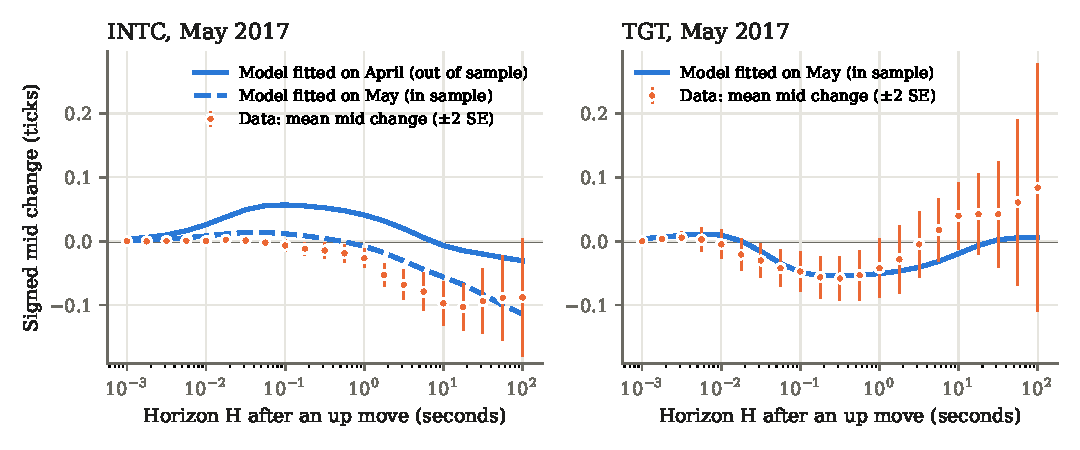
\includegraphics[width=\textwidth]{fig_response.pdf}
\caption{Signed mid-price change after clean up moves, May 2017. Points: realized change of the NBBO mid from the move to $H$ later (mean over moves within a day, then over days; bars $\pm 2$ day-clustered standard errors). Lines: the model's forecast given the signed accumulators just after each move (its actual history), averaged the same way. Script: \file{docs/overview/figures/make\_response\_figure.py}.}
\label{fig:response}
\end{figure}

\begin{itemize}
\item \textbf{TGT:} the in-sample model tracks the realized path from $1\ms$ to $1\sx$, including the reversal of about $0.06$ ticks at $0.1$--$1\sx$; beyond $10\sx$ the data continue more than the model (within wide error bars).
\item \textbf{INTC:} the May (in-sample) model tracks the path, including the reversal of about $0.1$ ticks at $10$--$60\sx$. The April model (out of sample) predicts a continuation of up to $0.05$ ticks at $0.1\sx$ that May does not show, and a smaller reversal. So the fast signed component did not carry over from April to May, while the slow reversal did, in sign if not in size.
\end{itemize}

\subsection{Backtest: INTC, out of sample}
\label{sec:res-oos}

Kernel fitted on April, tested on May; clean rule with $1\ms$ confirmation delay and $2\ms$ execution latency.

\begin{table}[ht]
\centering
\small
\begin{tabular}{@{}llrrrr@{}}
\toprule
Decision time & Deadline & Buy now & Wait to deadline & One-step rule & Share of deadline waited \\
\midrule
Random & $1\sx$ & $-0.000$ & $-0.002$ (0.002) & $\mathbf{-0.005}$ (0.001) & 0.49 \\
Random & $10\sx$ & $-0.000$ & $+0.004$ (0.004) & $\mathbf{-0.012}$ (0.003) & 0.45 \\
Random & $60\sx$ & $-0.000$ & $+0.001$ (0.014) & $\mathbf{-0.040}$ (0.011) & 0.33 \\
After up & $1\sx$ & $-0.000$ & $-0.017$ (0.009) & $-0.000$ (0.001) & 0.00 \\
After up & $10\sx$ & $-0.000$ & $-0.089$ (0.021) & $\mathbf{-0.073}$ (0.019) & 0.63 \\
After up & $60\sx$ & $-0.000$ & $-0.068$ (0.039) & $\mathbf{-0.155}$ (0.028) & 0.44 \\
After down & $10\sx$ & $-0.002$ & $+0.094$ (0.019) & $+0.009$ (0.003) & 0.05 \\
After down & $60\sx$ & $-0.002$ & $+0.208$ (0.038) & $+0.007$ (0.007) & 0.06 \\
\bottomrule
\end{tabular}
\caption{INTC, May 2017, kernel fitted on April. Mean cost in ticks (day-clustered SE). 14,432 random decisions, 7,925 after up moves, 7,929 after down moves. File: \file{results/INTC\_E1m\_test201705\_fit201704\_lag1ms\_lat2ms.csv}.}
\label{tab:oos}
\end{table}

\begin{itemize}
\item At random times the rule saves $0.040$ ticks with a $60\sx$ deadline: 8\% of the half-spread of $0.5$ ticks. Buying at once and waiting to the deadline both cost about zero on average.
\item After an up move it waits through the reversal and saves $0.155$ ticks (31\% of the half-spread), twice what a fixed wait to the deadline saves.
\item After a down move it buys at once (waits 5\% of the deadline on average) and avoids the $+0.21$ ticks that waiting costs.
\item With a $1\sx$ deadline after up moves the April model's fast continuation makes the rule buy at once, giving up $0.017$ ticks that waiting would have saved: the cost of the unstable fast component (Section~\ref{sec:res-stability}).
\end{itemize}

\subsection{Latency: raw against clean}
\label{sec:res-raw}

The raw rule uses the \Eo{} fit (May, in sample) and sees every NBBO change at once ($\ell_I = 0$); costs are on the same quoted ask.

\begin{table}[ht]
\centering
\small
\begin{tabular}{@{}lrrrr@{}}
\toprule
& \multicolumn{3}{c}{Raw rule (\Eo)} & Clean rule (\Em) \\
\cmidrule(lr){2-4}\cmidrule(l){5-5}
Execution latency $\ell_E$ & $0$ & $0.5\ms$ & $2\ms$ & $0$ and $2\ms$ \\
\midrule
Random, $10\sx$ & $-0.063$ (0.004) & $-0.048$ (0.004) & $-0.008$ (0.003) & $-0.013$, $-0.012$ \\
Random, $60\sx$ & $-0.188$ (0.007) & $-0.148$ (0.008) & $-0.025$ (0.008) & $-0.041$, $-0.040$ \\
After raw up, $60\sx$ & $-0.004$ (0.001) & $+0.101$ (0.005) & $+0.419$ (0.005) & --- \\
After raw down, $60\sx$ & $-0.127$ (0.006) & $-0.060$ (0.007) & $+0.084$ (0.013) & --- \\
Buy at once after raw up & $0$ & $+0.104$ & $+0.418$ & --- \\
\bottomrule
\end{tabular}
\caption{INTC, May 2017. Raw rule in sample; clean rule out of sample (April fit). Mean cost in ticks (day-clustered SE).}
\label{tab:latency}
\end{table}

\begin{itemize}
\item \textbf{At zero latency the raw rule wins}, by $0.19$ against $0.04$ ticks at random times. A raw up move is often the bid rising to the ask (a lock); the ask then rises within about a millisecond, and the rule buys just before. This is the latency race in the brief states.
\item \textbf{By $2\ms$ the race is lost.} The raw rule's saving at random times falls to $0.025$ ticks, below the clean rule's $0.040$; after raw up moves, buying at once costs $0.42$ ticks, because by the time the order arrives the ask has moved.
\item \textbf{The clean rule does not depend on execution latency} between $0$ and $2\ms$ (changes under $0.002$ ticks). The $1\ms$ confirmation delay matters more: in sample, from no delay to $1\ms$ the cost at random times ($60\sx$) moves from $-0.033$ to $-0.038$ and after up moves ($60\sx$) from $-0.180$ to $-0.159$ (first prototype run, costs on the mid). The conclusions do not change.
\item This splits the short-horizon predictability of consolidated quotes into a part in the brief states, worth about $0.15$ ticks per order at zero latency and gone by $2\ms$, and a latency-free part in the clustering of persistent moves, worth about $0.04$ ticks at random times and $0.15$ after up moves.
\end{itemize}

\subsection{Several timescales against one}
\label{sec:res-instant}

The \emph{instant} rule stops when the current signed intensity is non-negative, $D = g^\top d \ge 0$: it uses the same fitted model but ignores how each component decays, which is the rule a one-timescale model gives.

\begin{center}
\small
\begin{tabular}{@{}lrr@{}}
\toprule
Decision time, deadline & One-step rule & Instant rule \\
\midrule
Random, $10\sx$ & $-0.012$ (0.003) & $-0.011$ (0.004) \\
Random, $60\sx$ & $-0.040$ (0.011) & $-0.026$ (0.008) \\
After up, $10\sx$ & $-0.073$ (0.019) & $-0.000$ (0.001) \\
After up, $60\sx$ & $-0.155$ (0.028) & $-0.000$ (0.001) \\
After down, $10\sx$ & $+0.009$ (0.003) & $+0.027$ (0.007) \\
After down, $60\sx$ & $+0.007$ (0.007) & $+0.073$ (0.015) \\
\bottomrule
\end{tabular}
\end{center}

\noindent Same setting as Table~\ref{tab:oos}. After an up move the fast continuation component dominates the current signed intensity, so the instant rule buys at once and misses the slower reversal; after a down move it waits on the fast component and pays for the slow reversal. The timescale structure, not just the model, carries the value.

\subsection{TGT}

TGT, May 2017, kernel fitted on May (in sample), $1\ms$ confirmation delay, $2\ms$ execution latency.

\begin{center}
\small
\begin{tabular}{@{}llrrr@{}}
\toprule
Decision time & Deadline & Buy now & Wait to deadline & One-step rule \\
\midrule
After up & $0.1\sx$ & $+0.002$ & $-0.051$ (0.015) & $\mathbf{-0.066}$ (0.018) \\
After up & $1\sx$ & $+0.002$ & $-0.085$ (0.047) & $\mathbf{-0.078}$ (0.021) \\
After up & $10\sx$ & $+0.002$ & $+0.033$ (0.023) & $\mathbf{-0.059}$ (0.022) \\
After up & $60\sx$ & $+0.002$ & $+0.090$ (0.061) & $\mathbf{-0.025}$ (0.014) \\
After down & $0.1\sx$ & $-0.020$ & $+0.060$ (0.034) & $-0.017$ (0.004) \\
After down & $10\sx$ & $-0.020$ & $+0.102$ (0.071) & $+0.010$ (0.016) \\
Random & $60\sx$ & $+0.000$ & $+0.026$ (0.026) & $\mathbf{-0.033}$ (0.015) \\
\bottomrule
\end{tabular}
\end{center}

\noindent After an up move with a $10\sx$ deadline the rule waits through the $40\ms$ reversal and buys before the $10\sx$ continuation ($-0.059$ ticks, against $+0.033$ for waiting to the deadline). With a sign-changing response the decision after an event depends on the deadline in a non-monotone way. After a down move, buying at once with $2\ms$ latency already costs $-0.020$ ticks (the price keeps falling over the fastest, $5\ms$, component). These are in-sample numbers; the out-of-sample panel will confirm or revise them.

\subsection{Corrections made along the way}

Two claims made while developing the idea turned out wrong and are recorded here.
\begin{itemize}
\item \emph{``A trader using raw-event intensities loses.''} At zero latency the raw rule wins (Section~\ref{sec:res-raw}). The correct statement is about latency.
\item \emph{``TGT is a counterexample to monotonicity of the rule in the state.''} The one-step rule is monotone in each signed accumulator for TGT too (Proposition~\ref{prop:sign}). What TGT shows is non-monotonicity of the decision after an event in the deadline, and that the rule is not a threshold in the scalar signed intensity.
\end{itemize}
The first prototype also took the mean move size from the test month (a small look-ahead); the package takes it from the fit month. The one-step rule depends only on the sign of the expected displacement, so its decisions are unaffected.

%==========================================================================
\section{Weaknesses and risks}
\label{sec:weak}

\begin{itemize}
\item \textbf{Small magnitudes.} Hundredths of a tick per order at random times; tenths after moves. The contribution is structural (the signed kernel, the shape of the rule, the latency decomposition), not a trading strategy, and should be framed so.
\item \textbf{Two stocks, two months, one side.} Everything so far is INTC and TGT, buys only, April--May 2017. The panel job extends this (Section~\ref{sec:todo}).
\item \textbf{One-step rule, not optimal.} The values are lower bounds; the optimal rule is RQ1.
\item \textbf{Execution model.} One unit, no impact, no fees or rebates; the quoted ask during locks may not be accessible; SIP timestamps lag exchange time by up to $0.4\ms$.
\item \textbf{Misspecification.} The clean model is rejected by calibrated KS tests in every stock (hawkes-taq section 15); up-move misfit is unexplained. The drift formula assumes the symmetric kernel and a shared baseline; with an asymmetric kernel the signed intensity depends on the unsigned accumulators and the drift no longer closes on $d$.
\item \textbf{Instability.} The fastest signed component changed between April and May for INTC, and the out-of-sample rule paid for it at short deadlines. The slowest component is biased down in the bootstrap and sensitive to the baseline specification.
\item \textbf{Multiple testing.} Many deadlines, decision sets and latencies; results should be reported for a pre-set grid, out of sample, with the full table.
\end{itemize}

%==========================================================================
\section{Work to be done}
\label{sec:todo}

\subsection{Done}
\begin{itemize}[label=\done]
\item Formulation (P1) and the signed-kernel reduction; closed-form drift (Proposition~\ref{prop:drift}), stability (Lemma~\ref{lem:stable}), the long-run identity (Proposition~\ref{prop:longrun}) and the sign of the response (Proposition~\ref{prop:sign}).
\item Package \file{stopping/} (drift, accumulators, backtest with information delay and execution latency, one-step and instant rules), scripts for monthly fits and backtests, tests.
\item Prototype: INTC (April $\to$ May, out of sample), INTC raw at three latencies, TGT (in sample); instant-rule comparison; expected against realized path (Figure~\ref{fig:response}).
\item Repository \file{hyoeun-lee/hawkes-stopping}; cluster job for the panel.
\end{itemize}

\subsection{Next, in order}
\begin{enumerate}[label=\arabic*.]
\item \textbf{Out-of-sample panel} (\file{scripts/cluster/oos\_panel.sbatch}): eight stocks, fit April $\to$ test May and fit May $\to$ test June, \Em{} and \Eo, latencies $0$, $0.5$, $2$, $5\ms$. Add the sell side (mirror image) and the instant rule to the job.
\item \textbf{Signed kernel across the hawkes-taq panel}: $g_k$, $G$ and $\|g\|_1$ for all 112 stock-months from the saved self and cross excitations, with bootstrap standard errors for May 2017 from the saved refits. Which components are stable in sign and size across months? This answers RQ4 and guides which components a robust rule should use.
\item \textbf{Optimal rule} (RQ1): regression Monte Carlo on paths simulated from the fitted model for INTC and TGT; compare with the one-step rule on the same paths and on data; measure the option value of waiting and its dependence on activity.
\item \textbf{Simulation benchmark} (RQ5): the one-step rule's value on data simulated from the fitted model against its value on real data, by deadline. The gap measures what misspecification costs.
\item \textbf{Robustness} (RQ5): $K = 3$ against $K = 4$; full (asymmetric) kernel through simulation; baselines of 60 minutes and one per day; the $2\ms$ merge threshold; exchange-timestamp NBBO.
\item \textbf{Latency curve}: costs for $\ell_E$ from $0$ to $10\ms$ for raw and clean rules; locate where the raw rule's advantage ends, by stock (Nasdaq-listed against NYSE-listed, since SIP latency differs by venue).
\item \textbf{Theory}: verify the PDMP dynamic programming setting; prove or refute the monotonicity conjecture; the one-step rule's exact region in the $K = 2$ case as an illustration.
\item \textbf{Literature check}: a systematic search for Hawkes-based execution timing and signal-driven optimal stopping, to confirm the positioning in Section~\ref{sec:bg-exec}.
\item \textbf{P2 data}: best sizes from \file{complete\_nbbo} (field names to check on WRDS) for the resting-order problem.
\end{enumerate}

\subsection{Writing and targets}
Candidate journals: \emph{SIAM Journal on Financial Mathematics} or \emph{Mathematical Finance} if RQ1 yields a structural theorem; \emph{Quantitative Finance} or \emph{Market Microstructure and Liquidity} for the empirical latency decomposition (RQ3) with the one-step rule. The decision depends on what the optimal-rule work gives.

%==========================================================================
\appendix
\section{Repository map}

\begin{center}
\small
\begin{tabularx}{\textwidth}{@{}p{6.4cm}L@{}}
\toprule
File & Contents \\
\midrule
\file{stopping/drift.py} & \file{SignedDrift} (signed kernel, closed-form expected displacement), \file{Accumulators} (signed accumulators by recursion) \\
\file{stopping/backtest.py} & Decision sets, now/wait/one-step/instant rules, costs on the quoted ask, summaries with day-clustered SE \\
\file{stopping/\_\_init\_\_.py} & Locates hawkes-taq (\file{HAWKES\_TAQ} or \file{../hawkes-taq}) \\
\file{scripts/fit\_month.py} & Fit one stock-month (\Em{} or \Eo), save fit and mean move size \\
\file{scripts/run\_backtest.py} & Backtest one stock-month with a given fit, information delay, latency and rule \\
\file{scripts/cluster/oos\_panel.sbatch} & Out-of-sample panel, eight stocks, 2017Q2 \\
\file{tests/test\_drift.py} & Closed form against matrix exponential and simulated cascades; accumulator recursion \\
\file{docs/problem\_statement.md} & Short problem statement \\
\file{docs/prototype\_201705.md} & Prototype results \\
\file{docs/overview/overview.tex} & This document; figure scripts in \file{docs/overview/figures/} \\
\file{results/} & Aggregate backtest results (per-day files are not committed) \\
\bottomrule
\end{tabularx}
\end{center}

\section{Notation}

\begin{center}
\small
\begin{tabularx}{\textwidth}{@{}p{3.2cm}L@{}}
\toprule
Symbol & Meaning \\
\midrule
$\varepsilon_m$ & Sign of move $m$: $+1$ up, $-1$ down \\
$\mu(t)$ & Baseline, one level per day and 30-minute bin, shared by both directions \\
$\beta_k$, $1/\beta_k$ & Decay rate and memory of component $k$ \\
$a_k$, $c_k$ & Self- and cross-excitation of component $k$ \\
$g_k = a_k - c_k$ & Signed kernel; $G = \sum_k g_k$, $\|g\|_1 = \sum_k |g_k|$ \\
$u_k$, $d_k$ & Unsigned and signed accumulators \\
$D = g^\top d$ & Signed intensity $\lambda_+ - \lambda_-$ \\
$M = -B + \beta g^\top$ & Mean dynamics of $d$; $B = \operatorname{diag}(\beta)$ \\
$W(H) = \int_0^H e^{Mr}dr$ & Cumulative response; expected displacement $s\,g^\top W(H)\,d$ \\
$s$ & Mean move size in ticks \\
$T$, $\theta$ & Deadline; remaining time \\
$\ell_I$, $\ell_E$ & Information delay; execution latency \\
$h$ & Merge threshold of \Em{} ($1\ms$) and refractory period $\delta$ \\
\bottomrule
\end{tabularx}
\end{center}

%==========================================================================
\begin{thebibliography}{99}
\small

\bibitem{alfonsi} Alfonsi, A. and Blanc, P. (2016). Dynamic optimal execution in a mixed-market-impact Hawkes price model. \emph{Finance and Stochastics} 20(1), 183--218.
\bibitem{almgren} Almgren, R. and Chriss, N. (2001). Optimal execution of portfolio transactions. \emph{Journal of Risk} 3(2), 5--39.
\bibitem{avellaneda} Avellaneda, M. and Stoikov, S. (2008). High-frequency trading in a limit order book. \emph{Quantitative Finance} 8(3), 217--224.
\bibitem{bacry2013} Bacry, E., Delattre, S., Hoffmann, M. and Muzy, J.-F. (2013). Modelling microstructure noise with mutually exciting point processes. \emph{Quantitative Finance} 13(1), 65--77.
\bibitem{bacry2016} Bacry, E., Jaisson, T. and Muzy, J.-F. (2016). Estimation of slowly decreasing Hawkes kernels: application to high-frequency order book dynamics. \emph{Quantitative Finance} 16, 1179--1201.
\bibitem{bank} Bank, P., Cartea, \'A. and K\"orber, L. (2023). Optimal execution and speculation with trade signals. arXiv:2306.00621 (revised 2024).
\bibitem{bremaud} Br\'emaud, P. and Massouli\'e, L. (1996). Stability of nonlinear Hawkes processes. \emph{Annals of Probability} 24(3), 1563--1588.
\bibitem{cjp} Cartea, \'A., Jaimungal, S. and Penalva, J. (2015). \emph{Algorithmic and High-Frequency Trading}. Cambridge University Press.
\bibitem{cjr} Cartea, \'A., Jaimungal, S. and Ricci, J. (2014). Buy low, sell high: a high frequency trading perspective. \emph{SIAM Journal on Financial Mathematics} 5(1), 415--444.
\bibitem{chatziandreou} Chatziandreou, K. and Karbach, S. (2025). Optimal execution in intraday energy markets under Hawkes processes with transient impact. arXiv:2504.10282.
\bibitem{chevalier} Chevalier, E., Hafsi, Y. and Ly Vath, V. (2024). Optimal execution under incomplete information. arXiv:2411.04616.
\bibitem{cst} Cont, R., Stoikov, S. and Talreja, R. (2010). A stochastic model for order book dynamics. \emph{Operations Research} 58(3), 549--563.
\bibitem{costadavis} Costa, O. L. V. and Davis, M. H. A. (1988). Approximations for optimal stopping of a piecewise-deterministic process. \emph{Mathematics of Control, Signals and Systems} 1, 123--146.
\bibitem{davis84} Davis, M. H. A. (1984). Piecewise-deterministic Markov processes: a general class of non-diffusion stochastic models. \emph{Journal of the Royal Statistical Society, Series B} 46(3), 353--388.
\bibitem{davis93} Davis, M. H. A. (1993). \emph{Markov Models and Optimization}. Chapman \& Hall.
\bibitem{desaporta} de Saporta, B., Dufour, F. and Gonzalez, K. (2010). Numerical method for optimal stopping of piecewise deterministic Markov processes. \emph{Annals of Applied Probability} 20(5), 1607--1637.
\bibitem{gueant} Gu\'eant, O. (2016). \emph{The Financial Mathematics of Market Liquidity: From Optimal Execution to Market Making}. Chapman \& Hall/CRC.
\bibitem{glft} Gu\'eant, O., Lehalle, C.-A. and Fernandez-Tapia, J. (2013). Dealing with the inventory risk: a solution to the market making problem. \emph{Mathematics and Financial Economics} 7(4), 477--507.
\bibitem{gugerli} Gugerli, U. S. (1986). Optimal stopping of a piecewise-deterministic Markov process. \emph{Stochastics} 19, 221--236. [Details to verify.]
\bibitem{hardiman} Hardiman, S. J., Bercot, N. and Bouchaud, J.-P. (2013). Critical reflexivity in financial markets: a Hawkes process analysis. \emph{European Physical Journal B} 86, 442.
\bibitem{hawkes} Hawkes, A. G. (1971). Spectra of some self-exciting and mutually exciting point processes. \emph{Biometrika} 58(1), 83--90.
\bibitem{lallouache} Lallouache, M. and Challet, D. (2016). The limits of statistical significance of Hawkes processes fitted to financial data. \emph{Quantitative Finance} 16(1), 1--11.
\bibitem{leelee} Lee, H. and Lee, K. (2026). A spread-gated Hawkes-flocking model for best bid and ask dynamics, with an application to limit order placement. arXiv:2609.36631.
\bibitem{lee2023} Lee, Kyungsub (2023). Multi-kernel property in high-frequency price dynamics under Hawkes model. \emph{Studies in Nonlinear Dynamics \& Econometrics} 28(4), 605--624. arXiv:2302.11822.
\bibitem{leeseo2017} Lee, K. and Seo, B. K. (2017). Modeling microstructure price dynamics with symmetric Hawkes and diffusion model using ultra-high-frequency stock data. \emph{Journal of Economic Dynamics and Control} 79, 154--183.
\bibitem{lehalle} Lehalle, C.-A. and Mounjid, O. (2016). Limit order strategic placement with adverse selection risk and the role of latency. arXiv:1610.00261 (published in \emph{Market Microstructure and Liquidity}; details to verify).
\bibitem{ls} Longstaff, F. A. and Schwartz, E. S. (2001). Valuing American options by simulation: a simple least-squares approach. \emph{Review of Financial Studies} 14(1), 113--147.
\bibitem{ozaki} Ozaki, T. (1979). Maximum likelihood estimation of Hawkes' self-exciting point processes. \emph{Annals of the Institute of Statistical Mathematics} 31(1), 145--155.
\bibitem{peskir} Peskir, G. and Shiryaev, A. (2006). \emph{Optimal Stopping and Free-Boundary Problems}. Birkh\"auser.

\end{thebibliography}

\end{document}
